\documentclass[12pt]{article}
\usepackage[utf8]{inputenc}
\usepackage[english]{babel}
\usepackage{bbding}
\decimalpoint
\usepackage[spanish]{babel}
\usepackage{amsmath}
\usepackage{amsthm}
\usepackage{amssymb}
\usepackage{graphicx}
\usepackage[margin=0.9in]{geometry}
\usepackage{fancyhdr}
\usepackage[inline]{enumitem}
\usepackage{float}
\usepackage{cancel}
\usepackage{minted}
\usepackage{bigints}
\usepackage{color}
\usepackage{xcolor}
\usepackage{subfig}
\usepackage{listingsutf8}
\usepackage{algorithm}
\usepackage{tocloft}
\usepackage[none]{hyphenat}
\usepackage{graphicx}
\usepackage{grffile}
\usepackage{tabularx}
\usepackage[nottoc,notlot,notlof]{tocbibind}
\usepackage{times}
\usepackage{color}
\definecolor{gray97}{gray}{.97}
\definecolor{gray75}{gray}{.75}
\definecolor{gray45}{gray}{.45}
\renewcommand{\cftsecleader}{\cftdotfill{\cftdotsep}}
\pagestyle{fancy}
\setlength{\headheight}{15pt} 
\lhead{Block ciphers}
\rhead{\thepage}
\lfoot{ESCOM-IPN}
\renewcommand{\footrulewidth}{0.5pt}
\setlength{\parskip}{0.5em}
\newcommand{\ve}[1]{\overrightarrow{#1}}
\newcommand{\abs}[1]{\left\lvert #1 \right\lvert}

\author{Reporte 1}
\usepackage{minted}
\setminted{
    style=emacs,
    breaklines=true
}

%Permite crear columnas en el documento
\usepackage{multicol} 
\usepackage{color}
\usepackage{comment}
\newcommand{\tabitem}{~~\llap{\textbullet}~~}
\newcommand{\subtabitem}{~~~~\llap{\textbullet}~~}

\usepackage{cmbright}                               % Font


\bibliographystyle{IEEEtran}
\begin{document}
		\begin{titlepage}
			\begin{center}
				
				% Upper part of the page. The '~' is needed because \\
				% only works if a paragraph has started.
				
				\noindent
				\begin{minipage}{0.5\textwidth}
					\begin{flushleft} \large
						
\includegraphics[width=0.3\textwidth]{../ipn.png}
					\end{flushleft}
				\end{minipage}%
				\begin{minipage}{0.55\textwidth}
					\begin{flushright} \large
						\includegraphics[width=0.7\textwidth]{../escom.png}
					\end{flushright}
				\end{minipage}
				
				\textsc{\LARGE Instituto Politécnico Nacional}\\[0.5cm]
				
				\textsc{\Large Escuela Superior de Cómputo}\\[1cm]
				
				% Title
				
				{ \huge Session 5: Block ciphers \\[1cm] }
				
				{ \Large Cryptography} \\[1cm]
				
				{ \Large Group: 3CM6 } \\[1cm]
				
				\noindent
				\begin{minipage}{0.5\textwidth}
					\begin{flushleft} \large
						\emph{Students:}\\
						
						\begin{tabular}{ll}
					     Nicolás Sayago Abigail\\
					     Naranjo Ferrara Guillermo\\
					     
					\end{tabular}
					\end{flushleft}
				\end{minipage}%
				\begin{minipage}{0.5\textwidth}
					\begin{flushright} \large
						\emph{Teacher:} \\
						Díaz Santiago Sandra  \\
					\end{flushright}
				\end{minipage}
				
				\vfill
				
				% Bottom of the page
				{\large March 14, 2019}
			\end{center}
		\end{titlepage}
	
	\tableofcontents
	\newpage
	
    % -------------------------------------------------------------------------------------
    %                                     TOPICS
    % -------------------------------------------------------------------------------------
    \section{About Data Encryption Standard}
        For DES, data are encrypted in 64-bit blocks using a 56-bit key. The algorithm transforms 64-bit input in a series of stepes into a 64-bit output. The same stepes, with the same key, are used to reverse the encryption. Thre are two inputs to the encryption function: the plaintext to be encrypted and the key. In the next example, the plaintet must be 64 bits in length and key is 56 bits in length. (Actually, the function expects a 64-bit key as input. However, only 56 of these bits are ever used; the other 8 bits can be used as parity bits or simply set arbitrarily)

        % Image of general deciption of DES encryption
        \begin{center}
            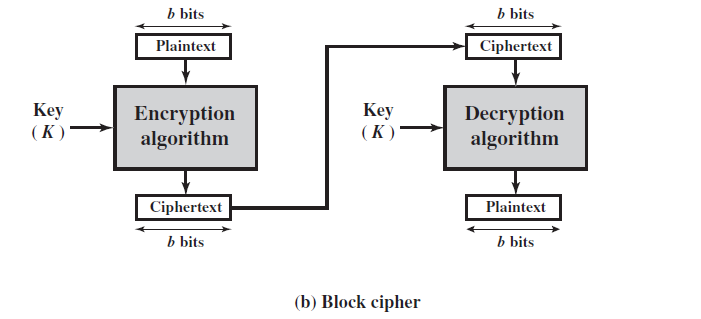
\includegraphics[width=0.9\textwidth]{Practica4/images/blockcipher.PNG}
        \end{center}
        
        Looking at the left-hand side of the figure, we can see that the processing of the plaintext proceeds in three phases.

        \subsection{Phase 1}
            The 64 bit plaintext passes through an initial permutation (\textbf{IP}) that rearranges the bits to produce the \textbf{permuted input}. 

        \subsection{Phase 2}
            Consisting of 16 round of the same function, which involves voth permutation and substitution functions. The ourtput of the last (16) round consists of 64 bits that are a function of the input plaintext and the key. The left and rght halves of the output are swapped to produce the \textbf{preoutput}.


        \subsection{Phase 3}
            The preoutput is passed through a permutation(IP$^{-1}$) that is the inverse of the initial permutation function, to produce the 64-bit ciphertext. With the exception of the initial and final permutations, DES has the exact structure of a Feistel cipher.

    \section{DES Decryption}
        As with any Feistel cipher, decryption uses the same algorithm as encryption, except that the application of the subkeys is reversed.
        dd

        \subsection{TripleDES}
            In essence involves repeating the DES algorithm three times on the plaintext using two or three diferente keys to produce the ciphertext.

    % -------------------------------------------------------------------------------------
    %                                     INSTRUCTIONS
    % -------------------------------------------------------------------------------------
    \section{Instructions}
        In this session we will use a cryptographic library to see how the blockciphers and the modes of operation work. To choose a cryptographic library, please only consider those that can be used with the programming languages: C, C++, Python, Java. To develop all the programming exercices you must use only one cryptographic library.

        \subsection{Programming exercises}
            Encipher and decipher files of different kind (.doc, .cpp, .java, .pdf, .jpeg, etc) using 3DES and different modes of operation. Consider the following requirements.

            \begin{numerate}
                \item Using a function to generate cryptographically pseudorandom generator, provided by the cryptographic library, generate a random key and store it in a file, using base 6, i.e. only use the characters A-Za-z0-9,+/. Consider that with 3DES the key size can be 112 and 160 bits. Try both sizes.

                \item To encipher, make proofs with the different alternatives we studied in class for 3DES: EEE and EDE with two and three keys. Also prove al the modes of operations CBC, CTR, OFB, CFB. Remember that the IV must be generated at random everytime you encipher a file. Generate the IV in the same way that you generate the key. Concatenate the IV with the ciiphertext and store them in a file.

                \item Find out which are the mechanisms are included in your library for padding. Choose one of them whenever is required to encipher your files. Avoid t use only zeros for padding.

                \item Decipher the files already encrypted.

                \item Use file of different sizes (500kb, 1MB, 5MB, 10MB). Please measure the execution time and make a graph to compare the execution time versus the file size, to encipher with the differente versions of 3DES with the differente modes of operation.

            \end{numerate}


    % -------------------------------------------------------------------------------------
    %                             LIST OF FUNCTIONS USED
    % -------------------------------------------------------------------------------------
    \section{Functions used}

        % ===============================
        %           FUNCTION 1
        % ===============================
        \subsection{Function 1 (NAME)}

            \begin{itemize}
                \item \checkmark\textbf{Param 1}
                \item \checkmark\textbf{Param 2}
                \item \checkmark\textbf{Param 3}
            \end{itemize}

        % ===============================
        %           FUNCTION 2
        % ===============================
        \subsection{Function 2 (NAME)}

            \begin{itemize}
                \item \checkmark\textbf{Param 1}
                \item \checkmark\textbf{Param 2}
                \item \checkmark\textbf{Param 3}
            \end{itemize}

    % -------------------------------------------------------------------------------------
    %                                     GRAPHS
    % -------------------------------------------------------------------------------------
    \section{Graphs}


    % -------------------------------------------------------------------------------------
    %                                     CONCLUSION
    % -------------------------------------------------------------------------------------
    \section{Conclusion}


    \section{Fuentes de consulta}
        %https://www.cryptopp.com/wiki/TripleDES
        %https://www.cryptopp.com/docs/ref/class_d_e_s___e_d_e2.html
        %https://www.cryptopp.com/docs/ref/class_auto_seeded_random_pool.html
            
\end{document}
 